\documentclass{article}
\title{中学数学やり直し — 文字式・方程式・関数}
\author{TeX 図書館}

\begin{document}

\section{この本の読み方 — やり直しの進め方}

中学数学は、解法を暗記してから忘れたときにこそ「そもそもなぜそうなるのか」が分からなくなります。本書は高校数学への接続を急がず、\textbf{式を変える理由からやり直す}ための本です。前提に必要なのは、中学校で習った用語と、正負の数の計算だけです。

つまずきは多くの場合、\textbf{符号の扱い}と、\textbf{等式の両辺を対称に変える操作}の 2 か所に集中しています。ここを直すと、方程式も関数も一緒に軽くなります。

\subsection{10 節の歩き方}

全 10 節は 3 つのまとまりに分かれます。

\begin{enumerate}
\item \textbf{第 2〜3 節 土台}: 正負の数と文字式。あらゆる計算の下敷きです。
\item \textbf{第 4〜7 節 主役}: 一次方程式・連立方程式・比例と反比例・一次関数。
\item \textbf{第 8〜10 節 応用と締め}: 図形の基礎、確率の基礎、次に進むための地図。
\end{enumerate}

順番に通読するのが基本ですが、「方程式だけ復習したい」という読み方も正しい使い方です。各節は独立して書かれており、必要な節だけを拾って構いません。

\begin{quote}
\textbf{【注意】}\ 本書が目指すのは\textbf{解法の暗記の回復}ではなく、\textbf{変形に理由が付けられる状態の回復}です。答えが合っているかより、途中の 1 ステップごとに「なぜ許されるか」を言えるかを手がかりにしてください。
\end{quote}

\subsection{変形は必ずルール付きで行う}

たとえば \(2x - 7 = 9\) を \(2x = 16\) に変えるとき、根拠は「両辺に 7 を足しても等しい」という一点だけです。式の変形は思いつきではなく、\textbf{宣言してから実行する一歩}になります。

\[ 2x - 7 = 9 \quad \Rightarrow \quad 2x = 16 \quad \Rightarrow \quad x = 8 \]

逆に、根拠を言えない変形はたいてい間違います。「なんとなく左辺を 2 で割った」で片側だけが変わるのが典型例です。本書ではすべての変形で、\textbf{いま使えるルール}を先に名指しします。

つまずきは、経験上 3 つに分かれます。

\begin{itemize}
\item \textbf{符号}: 引き算の符号を反転しない(第 2 節で扱います)。
\item \textbf{片側だけの操作}: 両辺に同じことをしていない(第 4 節)。
\item \textbf{式と言葉の往復}: 文章を式にしていない、式を言葉に戻せない(各節の末尾)。
\end{itemize}

「\(x\) の 2 倍から 7 を引いた数が 9」を式にしてみれば \(2x - 7 = 9\) です。文章題の入口は、この\textbf{翻訳}だけにあります。

\[ \frac{x}{2} + 1 = 4 \quad \Rightarrow \quad x = 6 \]

\textbf{解答の指針:}\ 各節末の問いでは、式を出す前に「その変形で使えるルールはどれか」を一言で言い当ててください。ルールを名指ししてから計算に移る習慣が、やり直しの第一歩です。

\section{正負の数 — 符号のきまりを一つにまとめる}

正負で迷うのは計算の手順ではなく、\textbf{符号をいつ反転するか}の一点です。増減・貸借・上下の違いをすべて吸収しているのが符号で、積と商のきまりは 1 行にまとまります。加法と乗法を分けて押さえます。

\subsection{加法と減法 — 引き算は足し算に帰着させる}

\(-5 + 3\) は「マイナス 5 に 3 加える」、\(-5 - 3\) は「マイナス 5 から 3 引く」。数直線上でどちらへ進むかだけの問題です。コツは、\textbf{引き算を符号反転した足し算}に置き換えることです。

\[ -5 - (-3) = -5 + 3 = -2 \]

向きがちがう数どうしを足すときは、絶対値の大きいほうから小さいほうを引き、結果の符号は大きいほうのまま残します。ここだけ守れば \((-9) + 4 = -5\) です。

\begin{quote}
\textbf{【定義】}\ 数 \(a\) の\textbf{絶対値} \(|a|\) は、数直線上で 0 からの距離です。符号とは独立に決まる大きさで、\(|-7| = 7\) となります。足し算の結果の符号は、この絶対値の大小で決まります。
\end{quote}

\subsection{乗法と除法 — 見るのは符号だけ}

積と商は「大きさの計算」と「符号の決定」が独立にできます。大きさは正の数のときと同じで、符号だけ次の表で決めます。

\begin{center}
\begin{tabular}{|c|c|c|}
\hline
 & 正の数 & 負の数 \\
\hline
正の数 & 正 & 負 \\
\hline
負の数 & 負 & 正 \\
\hline
\end{tabular}
\end{center}

\[ (-3) \times (-4) = 12 \qquad (-6) \div 2 = -3 \]

気温が 1 時間ごとに 3 度ずつ下がるとき、\(x\) 時間後の変化量は \(-3x\) です。\(x = 2\) なら \(-3 \times 2 = -6\) で、2 時間で 6 度下がります。符号は\textbf{下がる方向}を表す記号です。

計算に入る前、次の順に確認します。

\begin{enumerate}
\item \textbf{符号を先に決める}: 表か裏かの表で、積と商の符号を書きます。
\item \textbf{大きさだけを計算する}: 絶対値どうしの四則として普通に計算します。
\item \textbf{符号を戻す}: 手順 1 で決めた符号を結果に付けます。
\end{enumerate}

\textbf{解答の指針:}\ 「(-3) と (-4) の積は?」のような問いでは、値を出す前に「符号はどうなるか」を先に答えてください。表で符号を決め、残りは絶対値だけで計算します。符号と大きさを分けるのが正負のすべてです。

\section{文字式 — 変けられる数として式を見る}

文字式は、数の代わりに \(x\) や \(a\) を置いた式です。\(3 + 5 = 8\) は読み終えると何も残りませんが、\(a + b = b + a\) は\textbf{すべての場合}についての主張として残ります。ここに文字式の意味があります。

\subsection{たすきがけ — 展開の基本}

2 つの式を掛けるときは、左の各項を右の各項にかけ、その和を取ります。\((x + 3)(x + 5)\) では、\(x\) を通すと \(x^2 + 5x\)、3 を通すと \(3x + 15\) です。

\[ (x + 3)(x + 5) = x^2 + 5x + 3x + 15 = x^2 + 8x + 15 \]

中間の \(5x + 3x\) を \(8x\) にまとめるまでが展開です。ここを飛ばして \(x^2 + 15\) にする間違いが、文字式でもっとも多い失敗になります。

\subsection{因数分解 — 展開を逆にたどる}

因数分解は展開の逆で、和の形を積の形に戻す作業です。二次の式 \(x^2 + bx + c\) では、\textbf{積が \(c\)、和が \(b\)} になる 2 つの数を探します。

\[ x^2 + 7x + 12 = (x + 3)(x + 4) \]

\begin{quote}
\textbf{【注意】}\ \(x^2 + 7x + 12\) を \((x + 3)(x + 4)\) に戻せるなら、展開して確かめてよいです。\textbf{展開と因数分解は互いに検算できる}関係にあり、片方だけを信じる必要はありません。
\end{quote}

\(a^2 - b^2 = (a + b)(a - b)\) は展開・因数分解の両方で使う型です。\(9x^2 - 4 = (3x + 2)(3x - 2)\) のように、\textbf{形がそろえば}そのまま当てはめます。

頻出の型は次の 3 つだけです。

\begin{itemize}
\item \textbf{単項式 × 多項式}: 各項に掛けるだけ。\(3x(x + 2)\) なら \(3x^2 + 6x\)。
\item \textbf{多項式 × 多項式}: たすきがけ。項の組の数だけ積を作ります。
\item \textbf{特殊な型}: \(a^2 - b^2\) と完全平方。形を見て即座に当てはめます。
\end{itemize}

\textbf{解答の指針:}\ 因数分解の答えが出たら、必ず展開に戻して検算してください。\(x^2 + 7x + 12\) が \((x+3)(x+4)\) の積に戻ることを確かめられれば、その因数分解は完成です。戻せないなら、2 つの数の選び直しが要ります。

\section{一次方程式 — 両辺に同じことをする}

一次方程式とは、\(x\) の次数が 1 で \(ax + b = 0\) の形に整理できる式です。解く作業の正体はただ一つ、\textbf{両辺に対して同じ操作を繰り返して \(x\) だけを残す}ことです。

\subsection{等式の性質 — 変形の許可証}

等式は天秤と考えます。片側だけに何かを加えると倒れますが、両側に同じものを加えれば傾きは変わりません。

\begin{quote}
\textbf{【定義】}\ 等式 \(a = b\) に対し、両辺に同じ数を加える・引く・(0 でない数で)掛ける・割っても、等式は成り立ちます。一次方程式の変形はすべてこの 4 つから成り立ちます。
\end{quote}

\[ 2x - 7 = 9 \quad \Rightarrow \quad 2x = 16 \quad \Rightarrow \quad x = 8 \]

左辺の \(-7\) を消すために\textbf{両辺に 7 を足す}。このとき片側だけを操作すれば等式は壊れ、もとの解を見失います。

\subsection{移項と分数の消し方}

移項は「足し算を両辺から引く」の圧縮形です。\(3x + 5 = 20\) の \(+5\) を右へ移すとき、実体は両辺から 5 を引いているので符号が反転します。

\[ 3x + 5 = 20 \quad \Rightarrow \quad 3x = 15 \quad \Rightarrow \quad x = 5 \]

分数を含む式は、分母の最小公倍数を\textbf{両辺に掛ける}と消せます。\(\frac{x}{3} + 2 = 7\) は 3 を掛けて \(x + 6 = 21\)、よって \(x = 15\) です。「ある数に 5 を足して 2 倍すると 26」は \(2(x + 5) = 26\) と式化でき、\(x = 8\) が出てきます。

解き上げたら、最後に必ず\textbf{検算}します。もとの式に戻して左辺と右辺が一致すれば、その解は本物です。計算ミスの大半は、この 1 行を省いたときに見つかります。

手順にまとめると次の 3 段階です。

\begin{enumerate}
\item \textbf{整える}: 両辺を同じ形に寄せて、\(x\) の項と定数項を分ける。
\item \textbf{割る}: 係数で両辺を割り、\(x\) を単独にする。
\item \textbf{確かめる}: 解をもとの式に代入し、左右が等しいことを確認する。
\end{enumerate}

\textbf{解答の指針:}\ つまずいたら「いま \(x\) の前についているのは何か」を書き出してください。数字の足し算なら両辺から引き、掛け算なら両辺で割る。逆の操作を 1 つずつ適用すれば、\(x\) は必ず単独で残ります。

\section{連立方程式 — 2 つの未知数を同時に扱う}

未知数が 2 つあると、1 つの式だけでは絞り込めません。\(x + y = 10\) は \((1, 9)\) も \((7, 3)\) も満たします。\textbf{2 つの式を組み合わせて}初めて解が一意に決まります。

\subsection{代入法 — 表せる式から代入する}

どちらかの式で 1 つの文字をもう 1 つの文字で表せたら、その式をもう一方に代入します。\(y = 10 - x\) を \(x - y = 2\) に代入すると \(x - (10 - x) = 2\) となり、未知数が 1 つに減ります。

\[ x - (10 - x) = 2 \quad \Rightarrow \quad 2x - 10 = 2 \quad \Rightarrow \quad x = 6 \]

\(x = 6\) を \(y = 10 - x\) に戻せば \(y = 4\) です。\textbf{戻し算}まで終って初めて連立方程式は解けたことになります。

\subsection{加減法 — 足し合わせて消す}

片方の文字の係数をそろえ、式を足したり引いたりして消します。上の例では 2 式を足すだけで \(y\) が消えます。

\[ (x + y) + (x - y) = 10 + 2 \quad \Rightarrow \quad 2x = 12 \quad \Rightarrow \quad x = 6 \]

\begin{quote}
\textbf{【例】}\ 「大人 3 人分と子供 2 人分の料金が 3,200 円、大人 1 人分と子供 2 人分が 1,600 円」なら、2 式を引くと大人 2 人分が 1,600 円となり、大人 1 人分は 800 円です。\textbf{差を取る}のが加減法の典型です。
\end{quote}

代入法も加減法も、\textbf{「未知数を 1 つに減らす」という同じ目的}への別の経路です。どちらが速いかは式の形次第で、どちらを選んでも構いません。

判断は次の 3 行で終わります。

\begin{itemize}
\item \textbf{係数が 1 の文字がある} → その文字を式で表して代入法へ。
\item \textbf{係数が 2 式でそろっている} → 加減法で消します。
\item \textbf{どちらも違う} → どちらかの式を整数倍してから上に戻る。
\end{itemize}

解いたあとも、2 つの式に同じ \((x, y)\) を代入して\textbf{両方で成立するか}を確かめます。ここが連立方程式の検算です。

\textbf{解答の指針:}\ どちらの方法を選ぶかは「文字の係数が 1 か 0 か」で決めます。どちらかの文字の係数が 1 なら代入法、両方そろっているなら加減法。判断材料は式の見た目だけで足り、値を出す前には決められます。

\section{比例と反比例 — 比が一定か、積が一定か}

2 つの量の関係は、たいてい「比が一定」と「積が一定」のどちらかに分かれます。この 2 つを混同するとグラフを間違えるので、最初に切り分けます。

\subsection{比例 — 比が一定}

\(y\) と \(x\) の比が一定 \(k\) のとき、\(y = kx\) で表せて\textbf{比例}といいます。\(k\) は 1 単位あたりの量で、\(x\) を 2 倍にすれば \(y\) も 2 倍になります。グラフは原点を通る直線です。

\[ y = 3x \]

\(x = 5\) のとき \(y = 15\)、\(x = -2\) のとき \(y = -6\) です。比例は符号もそのまま引き継ぎます。

\subsection{反比例 — 積が一定}

\(y\) と \(x\) の積が一定 \(k\) のとき、\(y = \frac{k}{x}\) で表せて\textbf{反比例}です。\(x\) を 2 倍にすれば \(y\) は半分になり、グラフは原点をはさむ双曲線になります。

\[ y = \frac{12}{x} \]

\(x = 3\) のとき \(y = 4\)、\(x = 6\) のとき \(y = 2\) で、\(3 \times 4 = 6 \times 2 = 12\) が保たれます。

\begin{quote}
\textbf{【定義】}\ 比例は \(y \div x\) が一定、反比例は \(x \times y\) が一定です。\textbf{「どっちが一定か」}だけで区別でき、グラフが直線か曲線かもそこから決まります。
\end{quote}

2 つの量の関係を式にするときは、次の順で考えます。

\begin{enumerate}
\item \textbf{一定の量を探す}: 何が変わらず保たれているかを文中から拾います。
\item \textbf{形を決める}: 一定が比なら比例、積なら反比例と決めます。
\item \textbf{\(k\) を求める}: 1 組の値を代入して \(k\) を出し、式を完成させます。
\end{enumerate}

\textbf{解答の指針:}\ 問いを見たら「比が一定? 積が一定?」を先に答えてください。比なら \(k = y \div x\)、積なら \(k = x \times y\) を計算します。\(k\) が 1 つ求まれば、あとは式に流し込むだけです。

\section{一次関数 — グラフで読む関数}

一次関数は \(y = ax + b\) の形の関数で、グラフは直線になります。\(a\) は\textbf{傾き}、\(b\) は\textbf{y 切片}で、この 2 つの数が直線のすべてを決めます。

\subsection{傾きと切片}

傾き \(a\) は「\(x\) を 1 増やすと \(y\) がいくら増えるか」です。\(y = 2x + 1\) なら、\(x\) を 1 増やすごとに \(y\) は 2 増えます。

\[ y = 2x + 1 \]

\(x = 0\) のとき \(y = 1\) で、これが y 切片です。\(y = -x + 4\) なら傾きは \(-1\) で、右下がりの直線になります。

\begin{figure}
\centering
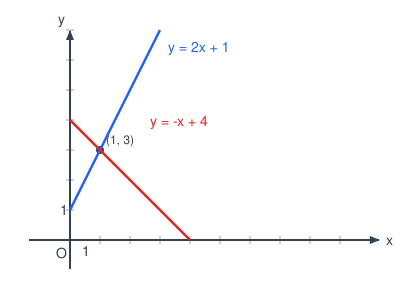
\includegraphics[width=0.8\textwidth]{figures/linear-graph.svg}
\caption{一次関数のグラフ}
\end{figure}

\subsection{2 つの点から式を求める}

グラフが 2 点を通るとき、傾きは \(a = \frac{y_2 - y_1}{x_2 - x_1}\) で求まります。点 \((1, 3)\) と \((2, 5)\) を通るなら \(a = 2\) です。

\[ a = \frac{5 - 3}{2 - 1} = 2 \]

あとは \(y = 2x + b\) に点 \((1, 3)\) を代入して \(3 = 2 + b\)、より \(b = 1\)。式は \(y = 2x + 1\) となります。

\begin{quote}
\textbf{【例】}\ 図の赤い直線は \(y = -x + 4\) です。青い直線 \(y = 2x + 1\) との交点は \(2x + 1 = -x + 4\) を解いて \(x = 1\)、\(y = 3\)。\textbf{交点の座標は 2 式の共通解}そのものになります。
\end{quote}

グラフから読むことは、この 3 つに尽きます。

\begin{itemize}
\item \textbf{切片}: 直線が y 軸と交わる点。\(x = 0\) での \(y\) の値です。
\item \textbf{増減}: 傾きが正なら右上がり、負なら右下がり。符号だけで決まります。
\item \textbf{交点}: 2 本の直線が出会う点。2 式の共通解で、どちらの式にも入っています。
\end{itemize}

\textbf{解答の指針:}\ 「直線が 2 点を通る」問題は、傾きの公式で \(a\)、代入で \(b\) の順に求めます。「直線同士の交点」問題は、2 式をつないで方程式に変えるだけです。図が見えたら、まず式に翻訳してください。

\section{図形の基礎 — 平行・垂直と角の関係}

図形の問題で理由を求められると苦しくなりますが、根拠は数個の\textbf{きまり}からしか出てきません。角の名前と、そのきまりを 3 つ押さえれば、証明は組み立てできます。

\subsection{平行線と錯角}

2 直線が平行なら、それらを横切る直線が作る\textbf{錯角}は等しく、\textbf{同位角}も等しく、隣り合う内角の和は 180 度です。逆も成り立ち、角の等しさから平行を言い合えます。

\begin{itemize}
\item \textbf{錯角}: 交点の対になる 2 つの角。平行なら等しい。
\item \textbf{同位角}: 同じ位置にあたる角。平行なら等しい。
\item \textbf{同側内角}: 横切る直線の同じ側にある内角。平行なら和が 180 度。
\end{itemize}

三角形の内角の和が 180 度であることは、平行線のきまりから導かれます。多角形は三角形に分割できるので、\(n\) 角形の内角の和は次の式で表せます。

\[ (n - 2) \times 180^{\circ} \]

六角形なら \((6 - 2) \times 180^{\circ} = 720^{\circ}\) です。分割の数だけ掛ける、という一本の筋に落ちます。

\subsection{垂直・二等辺三角形・三平方}

垂直なら交わる 4 つの角がすべて 90 度、二等辺三角形は底角が等しく、直角三角形では三平方の定理が働きます。

\[ 3^2 + 4^2 = 5^2 \]

二等辺三角形で頂角が 40 度なら、底角は \((180^{\circ} - 40^{\circ}) \div 2 = 70^{\circ}\) です。内角の和 180 度に\textbf{割り算を 1 回}するだけで終わります。

\begin{quote}
\textbf{【注意】}\ 「見えるから等しい」は理由になりません。\textbf{きまりの名前を添えて}「錯角が等しいから平行」「底角が等しいから」のように書く必要があります。図形の苦手さの多くは、手計算ではなくこの\textbf{名指し}の不足から来ています。
\end{quote}

\textbf{解答の指針:}\ 証明風の問いでは、「いま使っているきまりはどれか」を先に書き出してください。錯角・同位角・内角の和・底角・三平方の 5 つのうちどれかを名指せれば、あとは数値を流し込むだけです。

\section{確率の基礎 — 数えて、比べる}

確率は「好ましい場合の数」を「すべての場合の数」で割るだけです。むずかしいのは計算ではなく、\textbf{場合を漏らさず数える}ことにあります。

\subsection{数え上げの 2 つの法則}

同時に進む選択は掛け算、いずれかに分かれる選択は足し算です。飲み物が 2 種類、おやつが 3 種類なら、組合せは \(2 \times 3 = 6\) 通り。

\[ 2 \times 3 = 6 \]

サイコル 1 つの出方は 6 通りで、そのうち偶数が表れるのは 3 通りなので、確率は次の式で 1/2 になります。

\[ \frac{3}{6} = \frac{1}{2} \]

\subsection{確率の計算と補事象}

出方が等しく起きるときだけ、割り算が成立します。「表が出ない」は、表が出るほうの\textbf{反対}なので 1 から引けば足ります。

\[ 1 - \frac{1}{6} = \frac{5}{6} \]

\begin{quote}
\textbf{【例】}\ コインを 2 回投げる出方は 表表・表裏・裏表・裏裏 の 4 通りで、表と裏が 1 回ずつは 2 通りです。順序を区別して数えれば、確率は \(2 \div 4 = 1/2\) となります。
\end{quote}

割り算が使えるのは、次の 3 条件がそろったときだけです。

\begin{itemize}
\item \textbf{すべての場合を書き出せている}: 漏れも重複もなし。
\item \textbf{各場合が等しく起きる}: くじ引きのばらつきなどは除外します。
\item \textbf{分子はその一部}: 数えた「好ましい場合」が全体の数以下です。
\end{itemize}

\textbf{解答の指針:}\ まず「すべての場合」を書き出して数えてください。そこから「好ましい場合」を数え、割ります。割り算の前に\textbf{分母と分子を必ず口に出して数える}こと。等確率でなければ割り算できない、という落とし穴も同時に守れます。

\section{まとめと次の一歩 — 得た道具を棚に並べる}

10 節を終えると、中学数学の中心は「\textbf{変形のルール}」と「\textbf{一定の量}」の 2 つに集約されます。最後に、その棚を 1 枚の表に畳みます。

\subsection{覚えるべき型は 5 つ}

本書で使った型を、位置づけとともに挙げます。

\begin{center}
\begin{tabular}{|l|l|}
\hline
型 & 何が一定か / どこで使うか \\
\hline
正負の符号表 & 積と商の符号 \\
\hline
たすきがけと因数分解 & 展開と復元 \\
\hline
等式の性質 & 一次方程式の変形 \\
\hline
比例と反比例 & 比か積か \\
\hline
傾きと切片 & 一次関数の直線 \\
\hline
\end{tabular}
\end{center}

\(y = ax + b\) は、傾き \(a\) と切片 \(b\) を指定すれば直線が 1 本に決まります。逆に 2 点が分かれば \(a\) と \(b\) が決まる、という\textbf{双方向の関係}が一次関数の核心です。

\[ y = ax + b \]

\subsection{高校数学へつなぐ}

次に進むと、文字数が増えた式、次数が上がった式、関数の種類が増えていきます。その土台になる恒等式を 1 つだけ挙げておきます。

\[ (a + b)^2 = a^2 + 2ab + b^2 \]

\begin{quote}
\textbf{【注意】}\ やり直しは\textbf{終わりではなく停止点}です。解けるようになった実感が 1 つ積まれるごとに、次の節へ進める判断が付きます。詰まったら本書に戻ればよく、戻ること自体が失敗ではありません。
\end{quote}

進む順路の候補は、次の 3 つです。

\begin{enumerate}
\item \textbf{式がもどったら}: 因数分解と平方完成を足して、二次の式まで広げます。
\item \textbf{関数を深めたい}: 場合の数・データの見方へ進み、関数を「予測の道具」として使います。
\item \textbf{線を図形に戻したい}: 一次関数と直線の向きをつなげ、図形の証明へ移ります。
\end{enumerate}

\textbf{解答の指針:}\ 本書を閉じる前に、5 つの型を自分の言葉で 1 行ずつ説明できるか確かめてください。「何が一定か」「どちらへ変形してよいか」を言えれば、必要なら次の本に進んで構いません。言葉にできない型だけを、もう一度開いてください。

\end{document}
